\chapter{Introduction} \label{ch:introduction}

\section{Background}
An atomic nucleus consisting of neutrons and protons offers a laboratory to get insight into the nature of interactions lead by strong forces. These interactions are deciding factors for the structural arrangement of the nucleons in the nucleus as well as various decay mechanisms. The well-known decay mechanisms fall under the broad term radioactivity, which includes $\beta$-decay, $\alpha$-decay, $\gamma$-decay, and neutron/proton emission [reference]. A unique decay mechanism bearing a combination ($\beta$-decay and neutron emission) of radioactive decays  is called $\beta$-delayed neutron emission.

$\beta$-delayed neutron emission was first discovered in the context of nuclear fission in 1939 by R.B. Roberts et al. \citep{robert1939}. $\beta$-delayed neutron emission is a process observed in nuclei to the right of the line of stability, and gets more intense for (N/Z) $>>$ 1. Nuclei in this region are neutron-rich and neutron emission is expected to occur as we approach the neutron drip line. With an increase in $\beta$ decay Q-value (Q{\textsubscript{$\beta$}}) when going towards the neutron-rich region of the chart of nuclei, $\beta$\textsuperscript{-}-decay becomes the dominant decay mode. The daughter nucleus formed post $\beta$\textsuperscript{-}-decay is in an excited state and unstable against particle emission. The daughter nuclei, instead of deexciting through $\gamma$-ray emission can emit neutrons. Neutron emission may be the dominant mode of decay when the Q{\textsubscript{$\beta$}} value of the decay exceeds the neutron separation energy (S\textsubscript{n}) close to the neutron driplines. Figure \ref{fig:qb-sn} shows the values of (Q{\textsubscript{$\beta$}}-$S_{n}$) energy window for known nuclei, it keeps increasing as we have more and more neutrons in the system. Further, the populated states in the daughter nuclei can even lie higher than the two-neutron separation energy S\textsubscript{2n} enabling the emission of one or more neutrons.   

\begin{figure}[h]
	\centering
	\includegraphics[width=16cm, height=13cm]{figures/Qb_Sn.png}
	\caption[Q{\textsubscript{$\beta$}}-S{\textsubscript{n}} for nuclei in the chart of nuclei..]{Q{\textsubscript{$\beta$}}-S{\textsubscript{n}} for the known isotopes in the nuclear landscape. A higher value is seen for nuclei with large N/Z ratio far-off stability.}
	\label{fig:qb-sn}
\end{figure}  

Over the years, a number of nuclei were seen to exhibit this phenomenon. There are currently just over 200 nuclei with measured emission probability (P\textsubscript{xn}) values. However, a large number of nuclei are expected to engage in beta-delayed neutron emission as suggested by recent work of Moller \textit{et al.,} 2019 \citep{MOLLER20191}, here (P\textsubscript{xn}) values for nuclei spanning the chart of nuclei are predicted. The first observation of multi-neutron emission was seen for \textsuperscript{11}Li and it was identified to be a 2n emitter. $\beta$2n emission is mainly seen in nuclei lighter than Fe ranging from Li to K. \textsuperscript{86}Ga \citep{Yokoyama2018, 86Ga} stands as the strongest 2n emitter to date with measured 2n emission branching ratio of $\sim$ 15\%. \textsuperscript{100}Rb was known to be the heaviest $\beta$2n emitter with P\textsubscript{2n} value equal to 0.16(8)\%. Recent measurements for nuclei in A $\geq$ 100 have resulted in identifying \textsuperscript{136}Sb as a 2n emitter with a small P\textsubscript{2n} value of 0.14(13)\%. Three-neutron emission is theoretically predicted in the A$\geq$100 region of the nuclei chart \citep{MOLLER20191} but has never been experimentally measured. The P\textsubscript{1n} values are scarce for nuclei in the heavy mass region A$\geq$ 150 and no P\textsubscript{2n,3n} are known above mass A=100. 




Study of delayed neutrons is essential to a variety of fields ranging from nuclear structure and astrophysics to nuclear energy. With the advancement in the beam facilities enabling synthesis of nuclei in the \textit{terra incognito} region, coupled with advanced detectors and electronics, the study of such exotic nuclei is now possible. The $\beta$-decay properties of these radioactive isotopes give valuable information on nuclear structure/shell evolution in the regions far-off stability and provide input for astrophysical nucleosynthesis calculations. Several studies show peculiar structural aspects of nuclei solely from measured T\textsubscript{1/2} and P\textsubscript{n} values. One of these studies have hinted at single-particle structures and deformations in the ground state of Sr isotopes, mainly in the region 50$\leq$ N $\leq$ 60. Using $\beta$-delayed neutron emission branching ratios, $\beta$-decay strength distribution ($S_{\beta}$(E)) can be measured. Shifts in the value of $S_{\beta}$(E) have been linked to large deformations in \textsuperscript{42}Si \citep{n28}. Delayed neutron emission spectroscopy of \textsuperscript{83,84}Ga \citep{78Nimiguelmadurga} using VANDLE \citep{VANDLE} has revealed a prevalent mechanism of beta-delayed neutron emission in nuclei far from stability, giving strong evidence in support of Gamow-Teller transition, pertaining to large $S_{\beta}$(E) above the neutron-separation energy. Measurements on \textsuperscript{83,84}Ga also suggest \textsuperscript{78}Ni core excitation, leading to high neutron-emission branching ratios.

 

The $\beta$n-emission probabilities contain information about the structure of involved states and their energy differences. For the medium and heavy nuclei, the $P_{n}$ values show sensitivity to the competition between allowed Gamow-Teller(GT) and first-forbidden(FF) $\beta$-transitions caused by the ordering of the single-particle shell model states. The data regarding delayed-neutron branching ratios are also helpful to test the robustness of nuclear structure models far-off stability. The nuclei at and around shell gaps, e.g., in the doubly magic \textsuperscript{78}Ni region, are an excellent testing and development ground for a variety of physical models. Many of the r-process \citep{burdbidge}  nuclei are expected to be $\beta$-delayed two-neutron emitters, but the competition between $\beta$1n and $\beta$2n decay modes is not understood yet. The quantitative modeling of this effect requires the knowledge of the $\beta$-strength distribution, as well as a statistical model treatment of the competition between one- and two-neutron emission from the excited states in the daughter nucleus. The experiments include the direct $\beta$n branching ratio measurement in the decay of \textsuperscript{78}Ni$\textendash$the only particle-bound doubly-magic nucleus emitting $\beta$-delayed neutrons. A competition between one- and two-neutron emission has been hinted by Miernik \textit{et al.} \citep{86Ga} in the study of \textsuperscript{86}Ga. Results from the experiments at RIKEN are consistent with these measurements and bring about the incapability of the shell-model calculations to reproduce the $P_{1n, 2n}$ values. More data points in the region will help test the robustness of these models. The large decay strength deduced from the observed intense neutron emission is a signature of Gamow-Teller transformation. This observation was interpreted as evidence for allowed $\beta$ decay to \textsuperscript{78}Ni core-excited states, leaving the nucleus in the highly excited state because of the N = 50 shell gap. 


Further, there is great interest in $\beta$-delayed neutron-emission branching ratios of neutron-rich nuclei, which influence the final isotopic abundances of heavy isotopes during the late stages of rapid neutron capture r-process. A detailed study on the neutron energy and branching ratios can be a stepping stone to understanding the abundance patterns intensifying around the shell closures. Accurate and precise measurements of $\beta$-delayed neutron precursors are required to help improve nuclear physics inputs to modern r-process simulations with the aim of constraining the astrophysical site of the r-process. Experimental data on neutron-rich isotopes can also guide the development of quantified theoretical models capable of making reliable predictions for all nuclei involved in the r-process. Obtaining the critical experimental data will be part of an iterative process that requires close interaction between experimentalists, nuclear theorists, and astrophysicists.


\subsection{Present work}

The focus of the present work is on the research and development work done to develop a segmented-YSO based implantation detector, and experiment performed to study energy distribution of $\beta$-delayed neutrons in the \textsuperscript{78}Ni region using VANDLE. The YSO detector was used alongside BRIKEN counter at RIBF. A variant of the detector was employed in synchronization with VANDLE for neutron energy measurements.

The focus of the present work is also on the VANDLE experiment performed at the Radioactive Ion Beam Factory (RIBF) present at RIKEN Nishina Center, Japan to measure $\beta$-decay strength distribution from neutron-unbound states for the isotopes in the region. The BigRIPS fragment separator present at the facility was used to filter out the reaction products of the 345 MeV/u  \textsuperscript{238}U with \textsuperscript{9}Be target. The experiment is the first endeavor to conduct such measurements in the region. The measurements from the VANDLE experiment will provide the feeding intensity from the excited states in the daughter nucleus, and compute the associated strength with those states.
The dissertation also contains the study of $\beta$-decay of neutron-rich $\textsuperscript{79,80,81}$Cu isotopes decay and comparison with shell-model calculations. 




\section{$\beta$-decay}
The $\beta$-radioactivity was discovered as one component of the natural radioactivity (with $\alpha$ and $\gamma$ components) in the turn of the 20th century. The first experimental observations of this process were electrons emitted from radioactive sources. Further studies showed that the electron energy spectrum was continuous, and that $\beta$-decay seemed to violate conservation laws of nuclear physics (in particular energy, spin, and parity). The experimental observations convinced W. Pauli in 1930 to propose the emission of a second particle simultaneously with the electron, with negligible mass, no electrical charge, spin 1/2 and positive parity. This particle was called later the neutrino, and its experimental evidence was achieved in 1956. 
$\beta$-decay in general described as a process where a nucleus having Z protons and N neutrons decays to a nucleus having the same mass number A but with (Z $\pm$1, $N\mp$ 1). A $\beta$\textsuperscript{-}-decay may be regarded as the transformation of one of the protons to a neutron, and $\beta$\textsuperscript{+}-decay as that of one of the neutrons to a proton.
\begin{equation}
\textbf{$\beta$\textsuperscript{-} decay}: A(Z,N) \to A(Z + 1, N-1) + e\textsuperscript{-} + \overline{\nu}\textsubscript{e}
\end{equation}

\begin{equation}
\textbf{$\beta$\textsuperscript{+} decay}: A(Z,N) \to A(Z-1 , N+1) + e\textsuperscript{+} + {\nu}\textsubscript{e}
\end{equation}

Electron capture is another possibility where a nucleus captures an atomic electron. This process thereby changes a proton to a neutron and simultaneously causes the emission of an electron neutrino.
\begin{equation}
\textbf{Electron capture}:  e\textsuperscript{-} + A(Z,N) \to A(Z-1 , N+1) +{\nu}\textsubscript{e}
\end{equation}

Electron capture is mainly in competition with $\beta$\textsuperscript{+} decay and its probability is proportional to Z\textsuperscript{3} owing to increased Coulomb field and small electronic radius because of small electronic radius with increasing proton number in atoms.

\textbf{Q value} of a reaction is defined as the difference between the total kinetic energy before and after the reaction. 
\begin{equation}
Q = T\textsubscript{f} - T\textsubscript{i}
\end{equation}

Q values can further be expressed in terms of the atomic mass difference between parent and daughter nucleus. The expressions for Q-value for various decay types are listed as follows: 

\begin{equation}
\beta\textsubscript{-} decay:
Q\textsubscript{$\beta$\textsuperscript{-}} = (M(Z,N)  - M(Z-1,N+1))c\textsuperscript{2}  
\end{equation}

\begin{equation}
\beta\textsubscript{+} decay:
Q\textsubscript{$\beta$\textsuperscript{+}} = (M(Z,N)  - M(Z+1,N-1))c\textsuperscript{2} - 2m\textsubscript{e}c\textsuperscript{2}
\end{equation}

the 2m\textsubscript{e}c\textsuperscript{2} terms are used to compensate for the energy require to create a positron emitted and the atomic electron that must be ejected in going from a neutral atom of \textbf{Z} electrons to one with \textbf{Z-1} electrons
\begin{equation}
Q\textsubscript{EC} = (M(Z,N)  - M(Z+1,N-1))c\textsuperscript{2}-B\textsubscript{e}
\end{equation}
where B\textsubscript{e} is the ionization energy of the captured electron.

Nuclear $\beta$-decay was explained as a process undergoing weak interaction by Enrico Fermi \citep{fermitheory} in 1933. \textbf{Transition rate for $\beta$-decay} can be formulated using the Fermi's golden rule formulation, where a transition rate depends upon the strength of the coupling between the initial and final state of a system and upon the number of ways the transition can happen (i.e., the density of the final states)

\begin{equation}
\lambda = \frac{2\pi}{\hbar}|\langle\phi_{k}(r)|H^{'}|\phi_{o}(r)\rangle|^2\rho(E_{f})
\end{equation}

where $\rho$ (E\textsubscript{f}) is the density of final states and $H^{'}$ is the perturbation instigating the transition with $\phi\textsubscript{k}(r)$ and $\phi\textsubscript{o}(r)$ describing the entire initial and final states of the system, respectively. A formulation to determine the strength and the form is needed. The quantum mechanical problem can be broken into two parts: first to identify the matrix elements involved and second to determine the density of final states.

The initial state is characterized by the properties of the parent nucleus (spin, parity), and we assume it to be at rest. The final state is a combination of three particles, a neutral lepton(neutrino/anti-neutrino), a charged lepton (electron/positron), and the daughter nucleus. Considering all the prior statements the decay rate can be written in the form of an integral.

\begin{equation}
\lambda = \frac{g^2 |M_{fi}|\textsuperscript{2}}{2\pi^3\hbar^7c^3}\int_{0}^{p_{max}} F(Z_{D},p_{e})p_{e}^2(Q-T_{e})^2dp_{e}
\end{equation}

Here $|M_{fi}|^2$ is a nuclear matrix element representing the overlap between the initial and final	
nuclear states, g is the strength parameter, $p_{e}$ is the electron momentum, and $T_{e}$ is the electron kinetic energy. $\beta^{+}$-particles will be repelled by the nucleus, and their energy spectra are shifted to higher energy side while $\beta^{-}$-particles will be attracted and slowed down. These effects are incorporated by implementing the coulomb distorted wave functions and are contained in a spectrum distortion expression called the Fermi function, $F(Z_{D},p_{e})$, where $Z_{D}$ is the atomic number of the daughter nucleus. Equation 9.0 can be written in a simplified way by writing the integration part as $f(Z_{D},p_{e})$, known as Fermi-integral. 

\begin{equation}
\lambda = \frac{g^2 |M_{fi}|\textsuperscript{2} m_{e}^5c^4}{2\pi^3\hbar^7}f(Z_{D},p_{e}) 
\end{equation}

or in terms of the half-life of the parent nucleus, $T_{1/2}$ 

\begin{equation}
fT_{1/2}= \ln2\frac{2\pi^3\hbar^7}{g^2 |M_{fi}|\textsuperscript{2} m_{e}^5c^4}
\end{equation}

The left-hand side of this equation is called the comparative half-life, or \textquotedblleft ft-value\textquotedblright   because this value can be measured in experiments and should only depend on the nuclear matrix element and the $\beta$-decay strength constant. Typical \textit{ft} values vary from $10^{3}$ s to $10^{22}$ s; therefore the base ten logarithm of this value or log-ft is usually given in the literature. 

The spin and parity of the nuclear states involved in the $\beta$-decay process play an important role. They will determine the type of transition corresponding to the decay, either \textit{allowed} transition or \textit{forbidden} transition, and indicate how \textquotedblleft fast\textquotedblright the transition is.

\subsubsection{Allowed Transitions}

The notation J\textsuperscript{$\pi$} is used in the following, where J is the total spin of the nucleus or particle, and $\pi$ is the parity associated to that state.\\ The selection rules for allowed transitions are as follows:
\begin{enumerate}
	\item Leptons  $L_{l}$   $\rightarrow$ 0 (no angular momentum carried by the leptons)
	\item Nucleus $\pi_{i}\pi_{f}$ = +1 (no parity change)
\end{enumerate}

Since the two leptons can couple to a total intrinsic spin S, and given the condition that they don’t carry angular momentum, the change in the total angular momentum of the nucleus is dictated by how the spins of the two leptons emitted couple with each other. When the spins of the leptons are anti-parallel the total spin $\vec{S}_{l}$ = 0, and only $\Delta\vec{J}$ = 0 is possible (which is a singlet state). The corresponding transitions are called \textit{Fermi} transitions or \textit{vector} transitions. On the other hand if the spins of the two leptons are aligned $\vec{S}_{l}$ = 1, leading to $\Delta$J = 0, $\pm$1 (triplet state). This type of transition is called \textit{Gamow-Teller} transitions or \textit{axial} transitions. 
\\

Transitions where the spins of the final and initial states are $J_{f} = J_{i} = 0$  $(0 \to 0)$ are pure Fermi transitions. Alternatively, transitions with $\Delta$J = $\pm$1 are called pure GT transitions. A particular case of Fermi transition occurs when the nucleon involved in the $\beta$-decay process does not change any of its quantum numbers. This corresponds to $0^{+} \to  0^{+}$ transitions, which is experimentally observed near the N = Z region. These transitions are labeled as \textit{super-allowed} and offer a fascinating scenario as transitions are completely independent of strong interactions. 

\subsubsection{Forbidden Transitions}
Forbidden transitions follow at least one of the following selection rules:
\begin{enumerate}
	\item Leptons $\to \vec{L}_{l} > 0$, (angular momentum carried by leptons) or,
	\item Nucleus $\pi_{i}\pi_{f}$ = -1 (change of parity)
\end{enumerate}

These transitions are called forbidden because they are highly suppressed compared to allowed transitions. Since the matrix element is squared in the determination of the decay constant, each unit of l that has to be carried by the leptons will suppress the decay constant by approximately a factor $10^{-4}$ compared to the case with l = 0.

Forbidden transitions are classified into two branches, unique and non-unique, depending on the changes of spin and parity of the nucleus involved in the $\beta$-decay. For unique transitions, it appears that only one matrix element contributes to the transition, whereas in non-unique cases, several matrix elements will be participating. So forbidden transitions can be \textquotedblleft unique first-forbidden,\textquotedblright \textquotedblleft non-unique first-forbidden,\textquotedblright \textquotedblleft unique second-forbidden.\textquotedblright

A range of \textit{log-ft} values is characteristic of the type of transition, being super-allowed, allowed or forbidden.


\section{Delayed Neutron Emission}

There are many techniques used to predict the P\textsubscript{n} values, including phenomenological \citep{Phenomenoliogical}, shell model \citep{shellmodelhalflives}, and macroscopic-microscopic theories \citep{pmollermacroscopic}. Properly designed models help to provide information for nuclei far-off the reach of beam facilities. The predictions from the theory can be tested against the experimental calculations. This may lead to a validation of the theoretical approximations and a scope to improve models is always there, given the discrepancies seen between predicted and measured results. Experimentally calculated P\textsubscript{n} values can be compared with predicted values, providing a basis for fine-tuning the physics involved in these models. This also forms a basis to study the nuclear structure aspects on a microscopic basis. 

$\beta$-delayed neutron emission is mainly theorized as a multistage process consisting of the $\beta$-decay of the precursor (A, Z), which results in feeding the excited states of the emitter nucleus (A, Z+1) followed by the $\gamma$ de-excitation to the ground state or neutron emission to an excited state or to the ground state of the final nucleus (A-1, Z+1), where Z is the atomic number and A is the mass number of the precursor. The modeling scheme can also be broken into various steps to achieve the final delayed neutron energy spectrum or emission probabilities. Estimates of the Q\textsubscript{$\beta$} value is done mostly by using Finite Range Droplet macroscopic model by Moller et al. \citep{FRDMmoller}. Quasi-particle Random Phase Approximation (QRPA) model can be used to calculate the $\beta$-decay matrix elements and subsequent $\beta$-strength functions.  


\begin{figure}[h]
	\centering
	\includegraphics[width=17cm, height=10cm]{figures/delayed_netron_emission_cascaade.png}
	\caption[Schematic of the combined QRPA+HF approach]{Schematic of the combined QRPA+HF approach. Initial population of the the daughter nucleus (Z+1, A) is determined by QRPA. Subsequent delayed neutron and $\gamma$-ray emission are handled in the HF framework and shown by solid and dotted lines respectively. The statistical decay is followed until all available excitation energy is exhausted, denoted by trailing dots \citep{moller2016}. }
\end{figure}

Theoretically, the two integral $\beta$-decay quantities, T\textsubscript{1/2} and P\textsubscript{n}, are intertwined via their definition in terms of the $\beta$-strength function S\textsubscript{$\beta$}(E),

\begin{equation}
1/T_{1/2}=\sum_{0\leq E_{i}\leq Q_{\beta}}S\textsubscript{$\beta$}(E)  \times f(Z,R,Q_{\beta}-E_{i})
\end{equation}
where R is the nuclear radius, $Q_{\beta}$ is the maximum $\beta$-decay energy, and $f(Z,R,Q_{\beta}-E_{i})$ the Fermi function. From this definition, $T_{1/2}$ may contain information about average $\beta$ feeding of a nucleus. However, since transition rates to the low-lying states are strongly enhanced by the phase-space factor of $\beta$-decay, f$\sim (Q_{\beta}- E_{i})^5$, the largest contribution to $T_{1/2}$ comes from decays to the lowest-energy resonances in $S\textsubscript{$\beta$}(E_{i})$; that is, from the (near-) ground state allowed Gamow-Teller (GT) or first-forbidden (ff) transitions.

The $\beta$-delayed neutron emission probability ($P_{n}$) is schematically given by 
\begin{equation}
P_{n}=\frac{\sum_{S_{n}}^{Q_{\beta}} S\textsubscript{$\beta$}(E)\times f(Z,R,Q_{\beta}-E_{i})}{\sum_{0}^{Q_{\beta}} S\textsubscript{$\beta$}(E)\times f(Z,R,Q_{\beta}-E_{i})}
\end{equation}
which defines $P_{n}$ as the ratio of the integral $\beta$ intensity to states above the neutron separation energy, $S_{n}$, to the total $\beta$ intensity. 

The above formulation to get the $P_{n}$ values is mentioned in the literature as '\textit{cutoff}' method. It neglects $\gamma$ competition and assumes that only the higher multiplicity neutron emission prevails in the energy regions open to multiple neutron-emission channels. Also, it ignores the possibility of competition between one- and two-neutron emission as suggested by T. Kawano \textit{et al.,} 2013 \citep{kwano2013}. In order to explain the 1n/2n competition, Mumpower \textit{et al.} \citep{moller2016} implemented Hauser-Feshbach (HF) statistical model with QRPA. This is achieved by first calculating the $\beta$-decay intensities to accessible states in the daughter nucleus using QRPA. The subsequent decay of these states by neutron or $\gamma$-ray emission is then treated in the statistical Hauser-Feshbach (HF) theory. 


\subsubsection{$\beta$-decay feeding intensity $(I_{\beta})$}
When a parent nucleus $\beta$ decays to the daughter nucleus, the occupation of states in the daughter nucleus is controlled mainly by the $\beta$-decay selection rules (wave-function overlaps), i.e, the structure of the parent and the daughter nuclei. The wavefunction overlap between the parent and the daughter states is called the reduced transition matrix element for transitions connecting the states. The energy difference between the states of the parent and the daughter nucleus is another reason, decay to ground state or to states having low energy is preferred. As a general view of the $\beta$ decay, Figure \ref{fig:strength_distribution} shows the decay of a nucleus, and a distribution of S\textsubscript{$\beta$}(E) is shown ranging with the excitation energy in blue. The figure demonstrates the manifestation of equation 1.12 in $\beta$-decay. The low-lying states in the daughter nucleus exhibit a smaller S\textsubscript{$\beta$}(E) due to lesser wavefunction overlap, but S\textsubscript{$\beta$}(E) starts to augment for states above S\textsubscript{n}. The S\textsubscript{$\beta$}(E) can also reach very high values outside the decay window, manifesting as large resonance, known as Gammow-Teller resonance (GTR). The final $(I_{\beta})$ at a given excitation energy is decided by a convolution of S\textsubscript{$\beta$}(E) and phase-space factor at that energy.


\begin{figure}[h]
	\centering
	\includegraphics[width=16cm, height=10cm]{figures/strength_distribution.png}
	\caption[]{A schematic showing the decay of a $\beta$-delayed neutron precursor and the associated strength at excitation energy. The phase-space factor curtails $I_{\beta}$ at high excitation energies and augments it at lower energy.   }
	\label{fig:strength_distribution}
\end{figure}



\section{\textbf{r-process} and its role in nucleosynthesis}
The synthesis of nuclei beyond iron is attributed to the capture of neutrons by seed nuclei under extreme conditions. The processes known to play an essential part in this phenomena are r-process (rapid) and s-process (slow) \citep{burbridge}, where neutron capture reaction rates are relative to the $\beta$-decay time scales. For r-process $\tau_{n}$ $\ll$ $\tau_{\beta}$, whereas for s-process its the opposite case $\tau_{n}$ $\gg$ $\tau_{\beta}$. Considering the time scales, neutron capture path in s-process is close to the line of stability, and the nuclei involved in due course can be easily studied experimentally. r-process, on the other hand, will proceed into the very neutron-rich side far from the valley of stability. Once the neutron flux is exhausted, the unstable nuclei will decay back to the line of stability forming the stable r-process nuclei. 

\begin{figure}[h]
	\centering
	\includegraphics[width=15cm, height=10cm]{figures/r_process_path_way.png}
	\caption[Nuclei chart showing color-coded regions of stability]{Nuclei chart showing color-coded regions of stability, $\beta$-decay, $\alpha$-decay, and the r-process path. The r-process nuclei abundance pattern overlaid on the top-left demonstrates the peaks near closed nuclear-shells (Magic numbers) \citep{newmagicnumbers}.}
	\label{fig:r_process}
\end{figure}
The r-process path connects the isotopes with the maximum abundance in each isotopic chain. $\beta^{-}$-decays transfer nuclei from one isotopic chain to the next and determine the speed of the process. Abundance peaks occur due to long $\beta$-decay half-lives where the flow path comes closest to stability(closed neutron shells). The knowledge of $S_{n}$ and $\beta$-decay half-lives is helpful in determining the shape of the abundance curves.

Given the conditions conducive to r-process, experimental measurements are very challenging. The experimental bottleneck of synthesizing nuclei in the unexplored region of the chart of nuclei has been recently unblocked by a few facilities, thereby opening a whole new window to a plethora of information regarding mass and half-lives about the participating elements.

One of the significant challenges of our day is the determination of the site or sites for the r-process and therefore the identification of the origin of more than half of all the elements heavier than iron. The answer is complex and highly intermingled between the astrophysics that describes the conditions of the relevant scenarios and the physics of nuclei that operates in those scenarios. The sites of r-process have not been unambiguously identified, but a large number of neutrons required on short time scales hints at large neutron densities which are seen in explosive environments. The two leading candidates are type II (core‐collapse) supernova explosions and neutron star mergers. A recent observation of neutron star merger GW170817 \citep{gw170817} in various regions of the electromagnetic spectrum helps to narrow r-process sites. The observations suggest that the later part of the light curve produced by the post-merging supernova is backed by the radioactivity of lanthanides produced by r-process. 

\section{Nuclear structure}


The models used to define the structure of a nucleus are broadly classified into two categories, collective or independent. Collective models assume that nucleons interact strongly in the nucleus and their mean free path is small, whereas, independent models assume that the nucleons interact under the realm of Pauli principle in the nuclear matter and this leads to a larger mean free path. Now, models such as liquid drop model (collective), provides a good description of average behavior occurrence of binding energy pertaining to odd-even behavior, but it does not provide with the explanation of appearance of magic numbers of nucleons. This is mainly due to a structure of shells that cannot be obtained by the liquid drop model. Hence, there is a need to treat nucleus as a quantum system to provide with a justification for this behaviour. 

Moving on to the Fermi Gas Model, which falls under the category of independent models, is based on the notion of nucleons moving freely in the nucleus due to the Pauli principle. A nucleon in the nucleus feels the force of attraction created by all the nucleons around it. The situation can be imagined as to be similar to a balloon, inside of which nucleons can move freely, but occupy different states. The Fermi gas model, despite its simplicity explains many of the nuclear properties, it explains the lesser number of proton compared to protons as we go from from low A to high A nuclei, which is due to shallowing of proton well because of the coulomb repulsion between protons. Another explained characteristic is the high abundance of even-even nuclei compared to odd-odd nuclei. This is explained by the possibility of an isolated neutron or protons (each in their respective potential wells) in odd-odd nuclei to crossover to the well of the other via $\beta$-emission, returning to stability.


The shell model also follows the idea of nucleons moving independently of each other in the nucleus similar to the Fermi gas model. The difference here from the Fermi gas model is the introduction of a central potential, similar to the potential that acts on electrons in an atom. The central potential is the average potential created by all the nucleons in a nucleus. A nucleon is thus under the influence of a potential created by the rest of the nucleons in the nucleus. The potential should be determined in such a way to best produce the experimental results.

To give a mathematical form to the shell model, the Hamiltonian of a system consisting of A bodies can be written as

\begin{equation}
H = \sum_{i}^{A} T_{i}(r_{i}) + V(r_{1},......,r_{A})
\end{equation}
where T is the kinetic energy operator and V the potential function.
Now, if the interaction is restricted to two body the Hamiltonian assumes the mathematical form as follows:

\begin{equation}
H = \sum_{i}^{A} T_{i}(r_{i}) + \frac{1}{2}\sum_{ji}^{}V_{ij}(r_{i},r_{j}),
\end{equation}
In the shell model construct, a nucleon $\textit{i}$ feels not just the potential $\sum_{j}^{}V_{ij}$, but a central potential $U(r_{i})$, that depends only on the coordinates of nucleon $\textit{i}$. This potential can be introduced in the Hamiltonian as follows:
\begin{equation}
H = \sum_{i}^{A} T_{i}(r_{i}) + \sum_{i}^{A}U(r_{i}) + H_{res},
\end{equation}

$H_{res}$ is called the residual interaction, its part of the potential V not incorporated in the central potential U.
\begin{equation}
H_{res} = \frac{1}{2}\sum_{ji}^{}V_{ij}(r_{i},r_{j}) - \sum_{i}^{A}U(r_{i}),
\end{equation}

The $H_{res}$ term is generally anticipated to have a very small/negligible contribution to the \textit{shell model Hamiltonian}. 

The shape of the central potential should capture the features of the nucleus, i.e, the potential being maximum at the core and gradually waning closer to the radius. A potential called "Woods-Saxon" form is generally used to capture the features mentioned. Its mathematically defined as:
\begin{equation}
U(r) = \frac{U_{0}}{1+exp(\frac{r-R}{a})} 
\end{equation}

where $U_{0}$, R, and a represent as potential well depth, radius of the nucleus, and surface thickness, respectively.

The Schrodinger equation with the Hamiltonian H can be solved numerically providing wave functions of protons and neutrons characterized by shell (n), orbital (l), and total angular momentum (j) quantum numbers.


\begin{figure}[h!]
	\centering
	\includegraphics[width=12cm,height=10cm]{figures/Wood_sxaon.png}
	\caption[Wood-Saxon and square well potential for a nucleus with A = 70, $U_{0}$=50 MeV, and a = 0.5 fm.]{Wood-Saxon and square well potential for a nucleus with A = 70, $U_{0}$=50 MeV, and a = 0.5 fm. The plots demonstrates the shape of the Wood-saxon potential (blue) when compared to a square well potential (red). }
	\label{fig:woods_saxon}
\end{figure}
A considerable improved in matching the results was provided upon the addition of a spin-orbit interaction term to the Hamiltonian. The spin-orbit interaction term removes the degeneracy in the total angular momentum state \textit{j}. 


\begin{figure}[h!]
	\centering
	\includegraphics[width=17cm,height=10.5cm]{figures/shell_model.png}
	\caption[Level scheme of the shell model showing the breaking of degeneracy]{Level scheme of the shell model showing the breaking of degeneracy in the energy levels due to the spin-orbit interaction term. There is an emergence of some new magic numbers in the shell closing such as 28 and 50. The level scheme is not concrete and is expected to change as per the nuclear potential chosen.}
	\label{fig:shell_structure}
\end{figure}
After the discussion on the structure of an atomic nucleus using Shell model, we can rehash that an atomic nucleus is a quantum many-body system whose constituent nucleons (protons and neutrons) are subject to complex nucleon-nucleon interactions that include spin- and isospin-dependent components. For stable nuclei, the seemingly emerging patterns in some observables, such as the shell closure for neutrons or protons in nuclei: N, Z = 8, 20, 28, 50, 82, 126 can be explained with great success using shell-model calculations. 
\begin{figure}[h!]
	\centering
	\includegraphics[width=14cm,height=14cm]{figures/be2_n_50.png}
	\caption[Systematics of the $2\textsuperscript{+}$ excitation energy  ]{Systematics of the $2\textsuperscript{+}$ excitation energy for a) stable istopes and b) all nuclei measurements upto 2016. pritychenko et al., 2016 }
	\label{fig:2_plus_excitation}
\end{figure}

The testing of the shell model has been predominantly for stable nuclei and their neighbouring isotopes. The dynamics of interaction of nucleons in a nuclei starts to take a different turn with the addition of more neutrons/protons, mainly due to N/Z ratio deviating heavily from one. The picture of nuclear structure is quite different for nuclei far-off stability, these nuclei are also termed as "exotic." These exotic nuclei imply atomic nuclei with an unbalanced N/Z ratio as compared to stable ones, thus losing binding energy due to a large difference in Z and N (Bethe and Bacher, 1936; von Weizsäcker, 1935). Relatively smaller binding energies mean that $\beta$-decay channels open up, proceeding towards more N/Z balanced systems and resulting infinite (often short, sub-second, milliseconds) lifetimes. The asymmetry in N/Z ratio along with an interplay of nuclear forces can lead to emergence of new shell closures and shape deformations. The phenomena of change in the orientation of nuclear orbitals with the addition of more neutron/protons in stable isotopes is called "Shell Evolution." 

As an example of the shell evolution, systematics of the first $2\textsuperscript{+}$ levels is shown in the Figure \ref{fig:2_plus_excitation}. Part (a) of the figure shows appearance of magic numbers as predicted by the shell model having higher first $2\textsuperscript{+}$ excitation energy. Part (b) of the figure shows the data for nuclei measured until 2016, highlighting a relatively high $2\textsuperscript{+}$ excitation energy not predicted by shell-model, and displays the effects of shell evolution in structural properties.

The questions surrounding patterns in structure beyond stability can be answered by exploring various types of nuclear forces. The effects of nuclear forces affecting the shell structure can be studies in terms of their monopole component ot play. The monopole matrix element of an interaction, $\hat V$ is defined as 

\begin{equation}
v\textsubscript{m;j, j'} = \frac{\sum_{k, k'}^{}\langle jkj'k'|\hat V|jkj'k'\rangle}{\sum_{k, k'}^{}1},
\end{equation}
where $\textit{j}$ and $\textit{j'}$  denote the single-article angular momentum quantum numbers with $\textit{k}$ and $\textit{k'}$ denoting their respective magnetic substate, and quantity $\langle ...|\hat V|...\rangle$ is anti-symmetric in nature as per Pauli exclusion principle. Equation 1.19 shows the averaging over all possible orientations of two interacting particles in orbitals $\textit{j}$ and $\textit{j'}$. The monopole component of $\hat V$ is written, for $\textit{j}$ $\not=$ $\textit{j'}$, as 

\begin{equation}
\hat v_{m; j, j'} = v_{m;j,j'}\hat n_{j} \hat n_{j'},
\end{equation}


where the $\hat n_{j} (\hat n_{j'})$ is the number operator of the orbits $\textit{j (j')}$. The monopole component of the operator $\hat V$, as shown above is the average of all effects of $\hat V$, and it depends only on the occupation number of the orbits involved. Using neutron-proton scheme monopole interaction can be used with the convention: $n_{j}$ and $n_{j'}$ as the occupation number for protons and for neutrons in the orbits, respectively.


The shift in the single-particle energy (SPE) of proton orbits ($\textit{j}$) with the addition of neutrons in orbits ($\textit{j'}$) due to the monopole interaction can be written as 

\begin{equation}
\Delta \epsilon_{j} = v_{m;j,j'}n_{j'}.
\end{equation}


Due to linerarity of the monopole interaction, the effect of the monopole interaction can be magnified to a large degree with the increase in occupation of nucleons in valence orbit $\textit{j'}$, when we move away from the stability towards the neutron-rich side. As an example, Figure \ref{fig:monopole_interaction} depicts the monopole interactions that can take place as we keep filling neutrons in the $1g\textsubscript{9/2}$ (N$>$40) state, lying above the N=40 core. Single-particle proton states for Z $>$ 28 can be filled in $2p\textsubscript{3/2}$, $1f\textsubscript{5/2}$, and $2\textsubscript{1/2}$. 

\begin{figure}[h!]
	\centering
	\includegraphics[width=10cm,height=9cm]{figures/monopole_text.png}
	\caption[A graphical demonstration of the monopole interaction between the neutron single-particle state ]{A graphical demonstration of the monopole interaction between the neutron single-particle state $1g\textsubscript{9/2}$ and the proton single-particle states $2p\textsubscript{3/2}$, $1f\textsubscript{5/2}$, and $2\textsubscript{1/2}$. The shift in the energy of the state $1f\textsubscript{5/2}$ is larger compares to the shift for $2p\textsubscript{3/2}$ and $2p\textsubscript{1/2}$ due to a large radial overlap ($\Delta l = 1$) between the $\textit{f}$ and $\textit{g}$ shells. }
	\label{fig:monopole_interaction}
\end{figure}
The residual interaction can also have contributions from the spin-isospin interaction {reference from otsuka paper 2013}, which explain the appearance of magic numbers at Z=14 and N = 16. The tensor force {reference from otsuka paper 2013} due to pion exchange is another contribution to the residual interaction that has been explored for some nuclei.

\subsection{Shell evolution of Cu isotopes}


The sections above lay the basic foundation of structure of a nucleus and its evolution upon stuffing it with more and more neutrons due to the the monopole part of the nuclear forces. Here we discuss the shell evolution of $\textsubscript{29}$Cu isotopes. Copper isotopes display a great deal of shell-migration due to monople interaction and also display display competition between single-partcile and collective modes at low excitation energies [shell quenching in \textsuperscript{78}Ni [5-7]]. The idea of migration of states was seeded with the observation of lowering of $5/2^{-}$ in \textsuperscript{73,71}Cu [shell quenching in \textsuperscript{78}Ni 8]. This lead to a belief that $5/2^{-}$ may eventually become ground-state in \textsuperscript{75}Cu. $5/2^{-}$ was later confirmed as the ground state in \textsuperscript{75}Cu via magnetic moment measurements in the copper chain [shell quenching in \textsuperscript{78}Ni [7]]. The inversion was also predicted to be prevalent in  \textsuperscript{77,79}Cu. Figure \ref{fig:5_2_sytematics} shows the trend in the energy of the $5/2^{-}$ and $3/2^{-}$ states with the increase in neutron number. The observed trends in the energy of the low-lying states also point to the questioning of the Z=28 shell gap. There have been suggestion of the thinning in the Z=28 shell-gap. Studies mentioned in [persistance of shell-gap [23,24]] suggest a weakening of the Z=28 shell gap but the idea could not be substantiated with experimental measurements. However, half-life measurements hint at the survival of \textsuperscript{78}Ni doubly-magic (Z=28; N=50) characteristics with first excited state at $\sim$ 2 MeV. $\gamma$-ray measurements of the \textsuperscript{80}Zn(\textit{p,2p})\textsuperscript{79}Cu at RIBF ascertained the persistence of Z=28 shell-gap [persistance of shell-gap]. The findings of the experiment suggest at considering $\textsuperscript{29}$Cu consisting of a $\textsuperscript{78}$Ni with a valence proton, as depicted in Figure \ref{fig:Cu79_cartoon}. \textsuperscript{78}Ni was eventually identified to be doubly-magic with its $2^{+}$ state lying at 2.6 MeV [nature article] using in-beam $\gamma$-ray spectroscopy of \textsuperscript{80}Zn(\textit{p,3p})\textsuperscript{78}Ni reaction. Now to have a rather much closer look at the structure of $\textsuperscript{29}$Cu, $\beta$-decay strength distributions will be a useful tool to identify the strongest connecting states and the occupation of protons in excited states above $1f_{5/2}$. Read miguel's paper and draw ideas 


\begin{figure}[h]
	\centering
	\includegraphics[width=14cm,height=10cm]{figures/Cu_5_2_sytematics.png}
	\caption[Systematics of the  $5/2^{-}$ and  $3/2^{-}$ for odd-even Cu isotopes. ]{Systematics of the  $5/2^{-}$ and  $3/2^{-}$ for odd-even Cu isotopes. create your own picture using the data. }
	\label{fig:5_2_sytematics}
\end{figure}


\begin{figure}[h]
	\centering
	\includegraphics[width=10.5cm,height=8cm]{figures/Cu79_cartoon.png}
	\caption[$\textsuperscript{29}Cu$ depicted as having a $\textsuperscript{78}Ni$ core]{$\textsuperscript{29}Cu$ depicted as having a $\textsuperscript{78}Ni$ core and a valence proton orbiting in the $1f_{5/2}$ state as a ground state. }
	\label{fig:Cu79_cartoon}
\end{figure}




gather Cu isotopes information and show shell-evolution 

shell gap persistence 

whats beyond N>50, n>52

define the research gaps and fill in the information and mostly what my works provides and how it pushes the envelope.



